
\section{Graph-text-grounded Question Generation}

\begin{figure}[t]
    % \includesvg[width=0.80\textwidth]{figures/architecture.svg}
    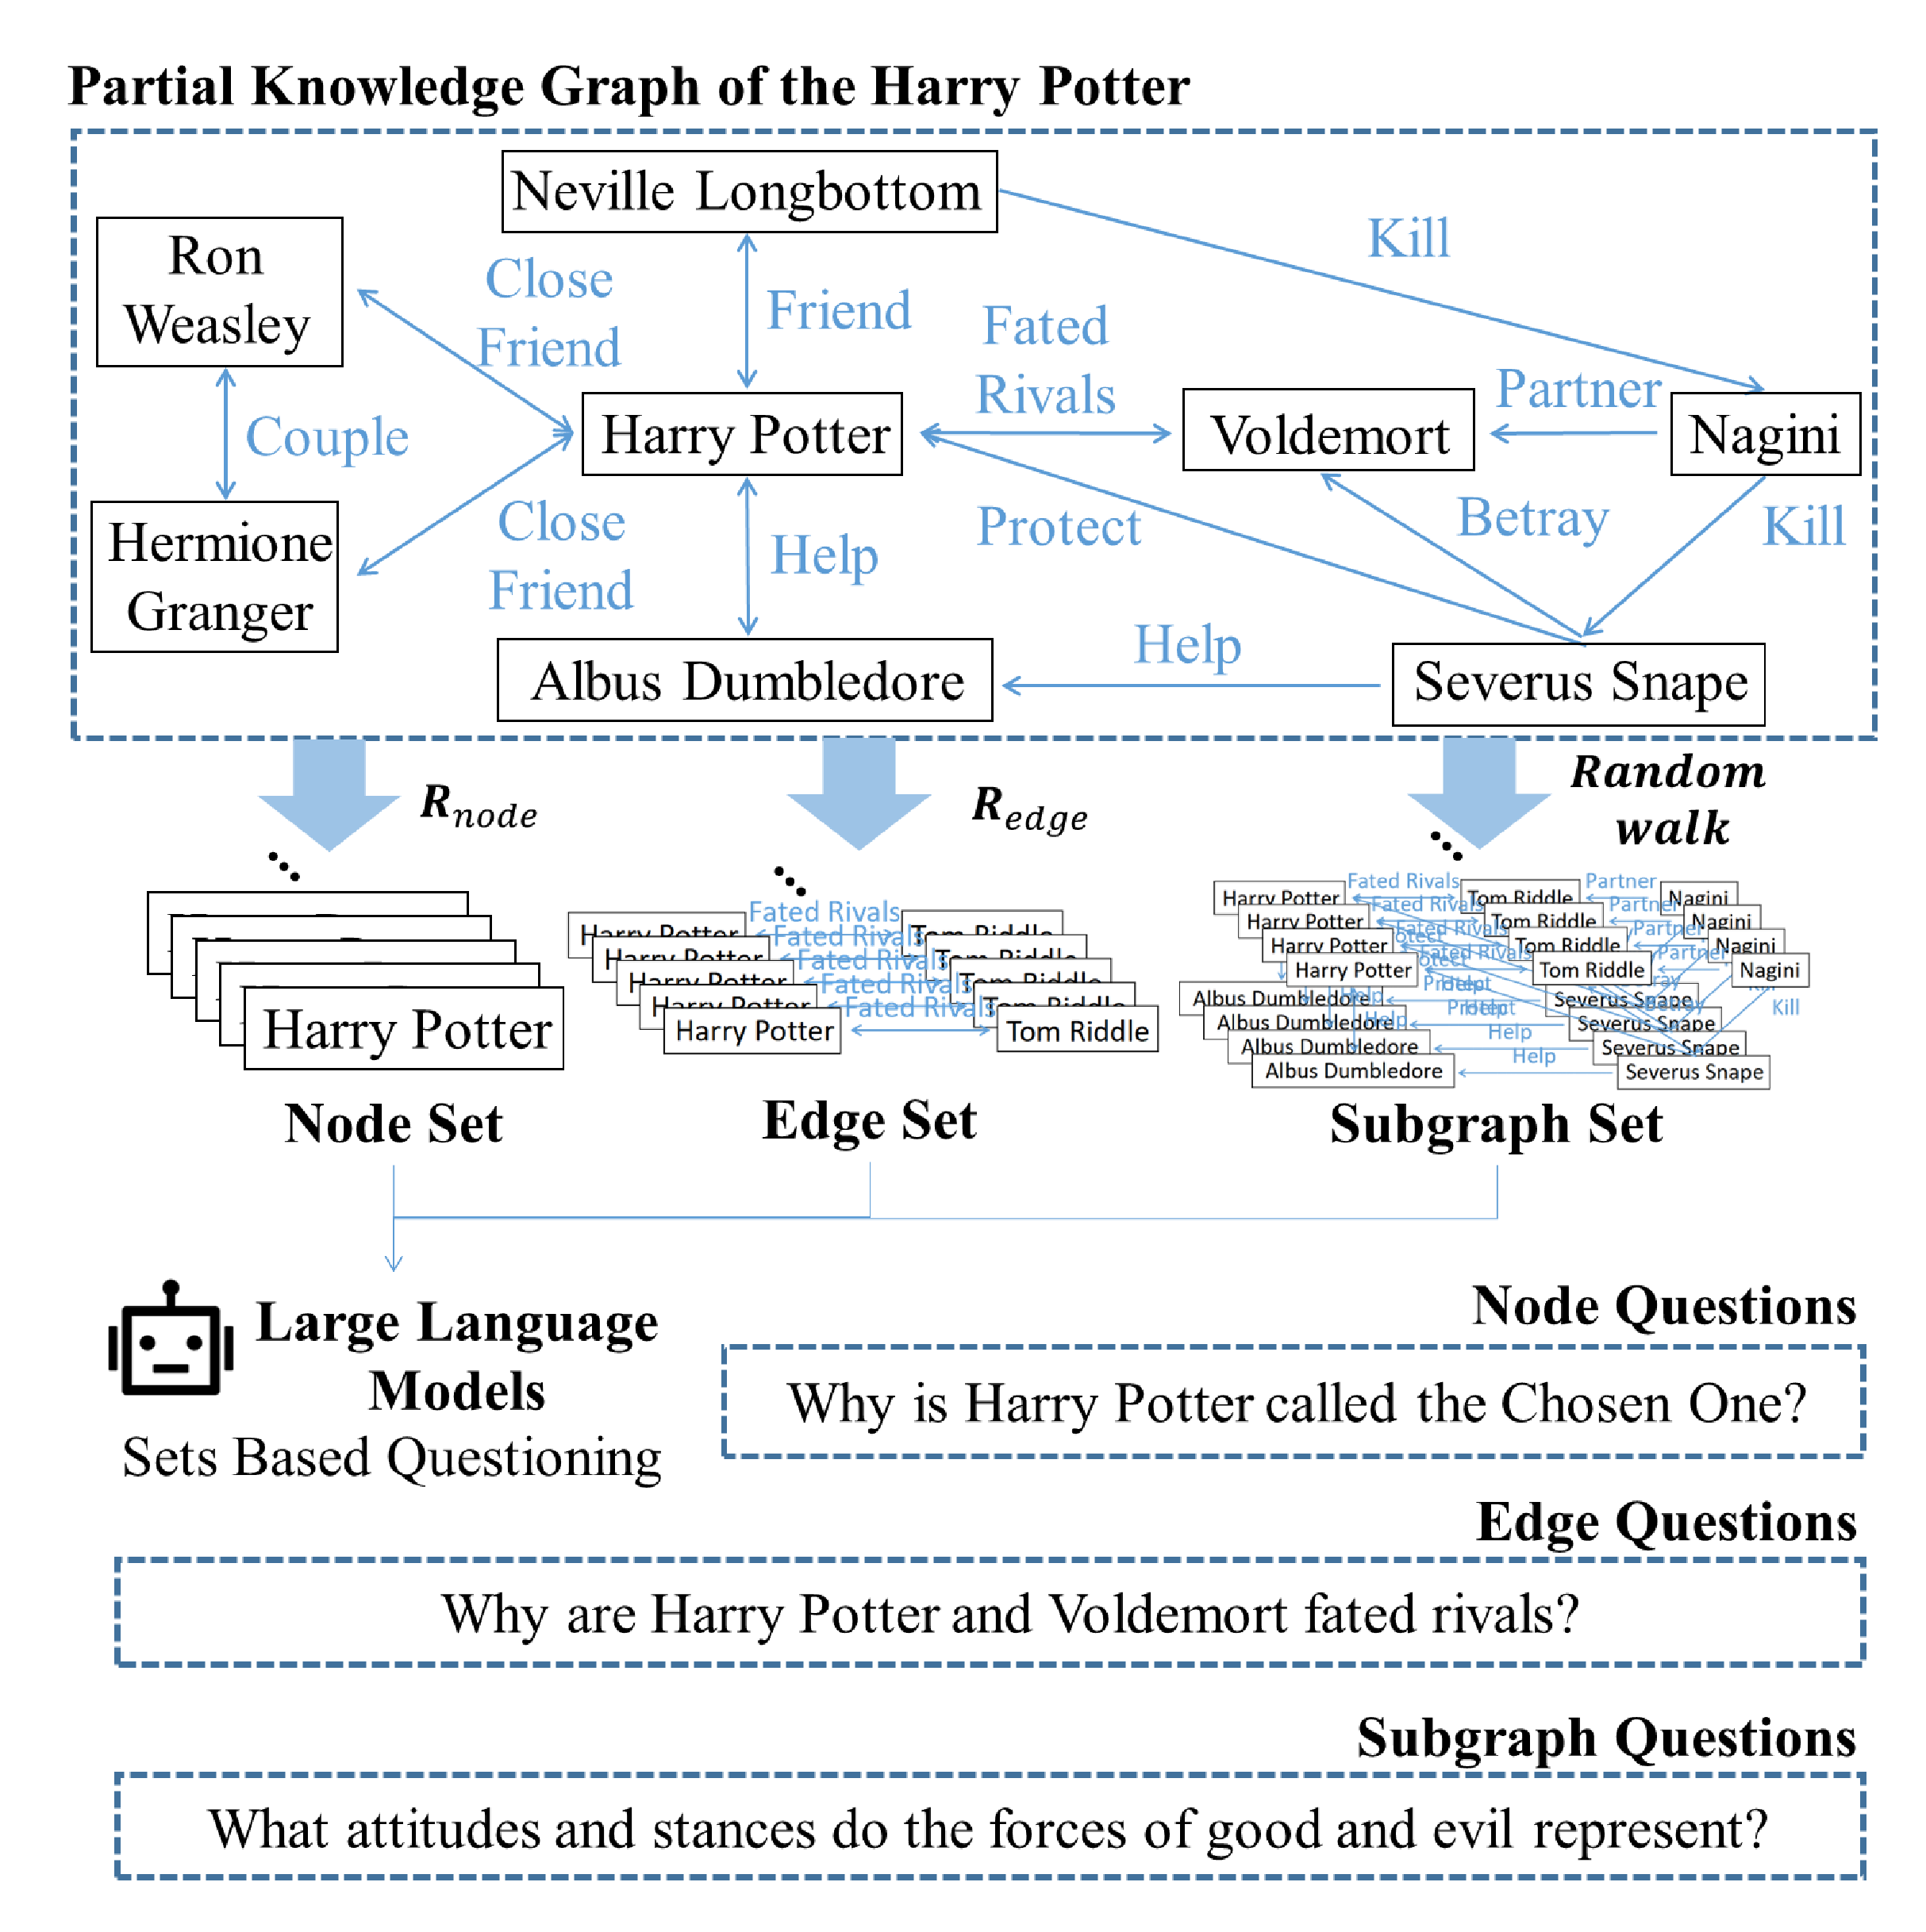
\includegraphics[width=0.5\textwidth]{pictures/ourquestion.pdf}
    \centering
    \caption{Workflow of graph-text-grounded question generation.}
    \label{fig:question}
\end{figure}



As shown in Figure~\ref{fig:introquestion}, the questions generated by the current summary-based method are too macroscopic to be answered using the dataset's knowledge or remain relevant. 
To tackle its defects, we propose a \textit{graph-text-grounded question-generation method}.

% Previous works like Graph RAG and Light RAG have used LLM for dataset question generation to test the system's answering capabilities. Their method is a summary-based question generation which involves directly splicing together the beginnings and ends of the articles in the dataset to create an overview, then stacking the overviews to develop a description of the dataset. This description is then used as an input to LLMs, which drives the LLMs to generate questions. This method can produce questions, but we find that the LLMs may provide poor-quality questions that are not highly relevant to the dataset's knowledge once given these extremely general and inaccurate descriptions. 

\stitle{Question Generation.}
Our graph-text-grounded question generation leverages the knowledge graph to produce questions that are closely related to the dataset.
This process consists of two steps: \textit{knowledge graph construction} and \textit{graph-text-grounded question generation}.

\squishlist
\item \textit{Knowledge graph construction}. We first segment the dataset articles into fine-grained chunks and employ an LLM to extract the entities and relations. 
We prompt the LLM to conduct deeper mining, e.g., using prompts like `\textit{identify the missing entities and add them}'. 
The extracted entities and relations are enriched with the descriptions derived from their source articles. 
These descriptions are stored in a knowledge graph, with the duplicate entities merged to maintain consistency and completeness.
After establishing the knowledge graph, we will associate each entity (node and relationship) in the knowledge graph with its corresponding original text paragraph to ensure that the source of the text paragraph is not lost.

\item \textit{Graph-text-grounded question generation}.
Figure~\ref{fig:question} shows our procedure for question generation. We leverage the knowledge graph to generate questions at three levels, i.e.,  \textit{node}, \textit{edge}, and \textit{subgraph}. At the node and edge levels, we conduct random sampling for the entities and relations of the knowledge graph. These sampled entities and relations form context structures, which are then used to prompt the LLM to generate questions. In particular, at the node level, we instruct the LLM to focus on the contents of the entities to generate relevant questions. At the edge level, we prompt the LLM to focus on the descriptions of the relations to propose inferential questions.
To prevent the quality of the knowledge graph itself from being strongly correlated with the quality of the problem, we will simultaneously take the original text segment corresponding to the entity as supplementary input. In this way, even if the quality of the knowledge graph itself has problems, it can still ensure to the greatest extent that the problem is faithful to the original text.
To generate subgraph-level questions, we first sample a node in the knowledge graph and perform random walk algorithm~\cite{li2015random} from the seed node to extract a subgraph with multiple walk steps. We enforce a minimum size threshold (which is 50 non-repeating hops in default) for the subgraph such that the subgraph encompasses rich entities and relations. If a sampled subgraph falls below the threshold, we resample to ensure adequate size. Given a subgraph, we use it to form context structures that guide the LLM in generating questions that require an overall understanding and reasoning about the subgraph.
For subgraph scenarios, we will first generate summaries of the text segments corresponding to all entities within the subgraph. Since the text segments involved in the subgraph at this time are far less than those directly generated for the full text, the summaries will be more accurate. Next, we use the generated summary as supplementary input to assist in generating subgraph-level questions.

% The question-generating LLM is instructed to identify N potential users and M tasks for each user and to generate K questions for each possible user-task combination. For our analysis, 50 test questions per level were generated with a setting of N = 5, M = 5, and K = 2.
\squishend

\begin{figure}[t]
    % \includesvg[width=0.80\textwidth]{figures/architecture.svg}
    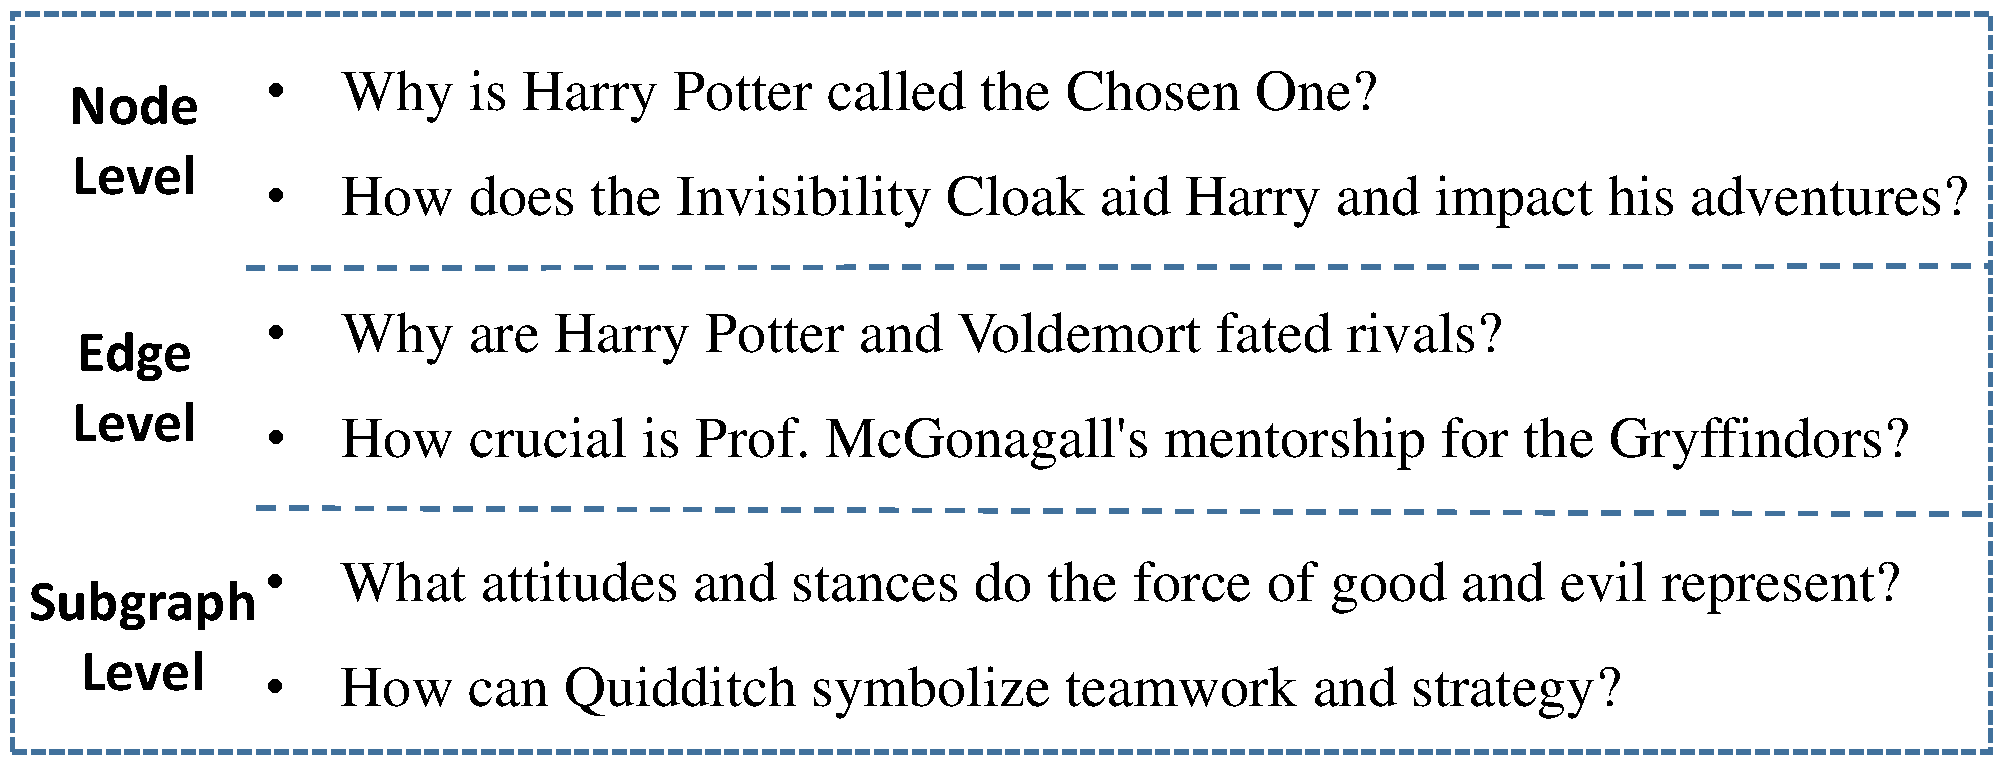
\includegraphics[width=0.5\textwidth]{pictures/myquestion.pdf}
    \centering
    \vspace{-2em}
    \caption{Examples of the questions generated by our graph-grounded method for the Harry Potter novel.}
    \label{fig:questionexample}
\end{figure}

\stitle{Question examples.}
We utilize the Harry Potter novel as the dataset to compare the questions generated by the existing summary-based method and our graph-text-grounded method. In particular, Figure \ref{fig:questionexample} shows the questions generated by our method, while Figure~\ref{fig:introquestion} shows the questions generated by the existing method. 
It can be observed that the summary-based method produces questions that are too dispersed and sometimes unanswerable or irrelevant given the underlying dataset. Take the last question in Figure~\ref{fig:introquestion} for example, it is evident that GraphRAG methods cannot forecast the box office receipts using knowledge from the Harry Potter novel. This is because the summary-based method relies on vague summaries of the articles and dataset, which lose the fine-grained details. This problem becomes more significant for larger datasets due to more articles and increased ambiguity.
% In contrast, our proposed graph-grounded question generation method excels at producing targeted questions across various graph levels. At the node level, it focuses on entity-specific details. At the edge level, it prompts reasoning about entity relationships, such as causality or correlation. At the subgraph level, it formulates broader questions that demand a comprehensive understanding of the graph's structure and semantics, assessing the synthesis of information across multiple nodes and relationships.
In contrast, our graph-text-grounded method produces questions that are closely related to multiple levels of the underlying dataset. At the node level, it generates questions focused on the attributes and characteristics of individual entities, testing the ability to retrieve detailed knowledge of specific nodes for GraphRAG methods. At the edge level, it creates inferential questions that explore relations between entities, such as causality or correlation, assessing relational reasoning abilities. At the subgraph level, it formulates macroscopic questions requiring a holistic understanding of multiple interconnected entities, evaluating the ability to synthesize information and comprehend broader structural and semantic contexts. 

% In contrast, our proposed graph-grounded question generation method is highly effective in generating questions across multiple levels of a graph structure. 
% Specifically, at the node level, our method produces questions that are specific to individual entities, focusing on their attributes, properties, and unique characteristics. These questions are designed to test the understanding of detailed information associated with each node.
% At the edge level, our method generates inferential questions that require reasoning about the connections and interactions between different entities. These questions probe the nature of the relationships, such as causality, correlation, or hierarchical dependencies, and assess the ability to infer information based on the links between nodes.
% At the subgraph level, our method creates more macroscopic questions that require a broader range of knowledge to answer. These questions involve multiple entities and their relationships within a larger context, necessitating an understanding of the overall structure and semantics of the sub-graph. They are designed to evaluate the ability to synthesize information from various parts of the graph and provide comprehensive answers based on a holistic view of the data.

% \zqm{this part can be longer if needed}

% Overall, our graph-grounded question generation method provides a comprehensive and multi-faceted approach to generating questions that can effectively assess the understanding and reasoning capabilities across different levels of a given dataset.